\subsection{Validazione e Collaudo}
\label{validazione_e_collaudo}
\textbf{Durata:} dal 2021\_04\_10 al 2021\_05\_09 \\
Il periodo di validazione e collaudo inizia appena concluso il precedente e termina con la \textbf{Revisione di Accettazione.}

Le precondizioni sono:
\begin{itemize}
    \item Le postcondizioni del periodo precedente sono state soddisfatte;
\end{itemize}

Le postcondizioni sono:
\begin{itemize}
    \item Aggiornamento e correzione documenti già prodotti;
    \item Esecuzione dei vari test;
    \item Completamento del prodotto in base a quanto discusso durante la \textbf{Revisione di Qualifica};
    \item Consegna dei documenti richiesti in entrata alla \textbf{Revisione di Accettazione};
    \item Ultimata preparazione della presentazione da esporre in sede di revisione.
\end{itemize}
E' composto da nove incrementi e una nuova attività:
\begin{itemize}
    \item \textbf{Incremento e Verifica dei documenti}: alcuni dei documenti già prodotti vengono migliorati e aggiornati (\textit{\NdP}, \textit{\PdP}, \textit{Glossario},\textit{\PdQ}, \textit{Specifica Tecnica}, \textit{Manuale Utente}); 
    \item \textbf{Incremento e Verifica delle Attività}: Se necessario vengono migliorate le attività di \textit{Technology Baseline} per quanto riguarda la progettazione ad alto livello, in particolare la \textit{Product Baseline} riguardo all'aggiunta di design pattern o di diagrammi di classi o di attività, la parte di \textit{Codifica}, in caso non siano stati riscontrati rallentamenti o ritardi nel progetto, potrebbe comprendere l'implementazione di uno o più casi d'uso opzionali.
    \item \textbf{Validazione e Collaudo}: Realizzazione degli ultimi test, con successivi controlli finali per garantire un buon livello di qualità e correttezza.
\end{itemize}

\newpage
\subsubsection{Diagramma di Gantt: Validazione e Collaudo}
\begin{figure}[ht]
    \centering
    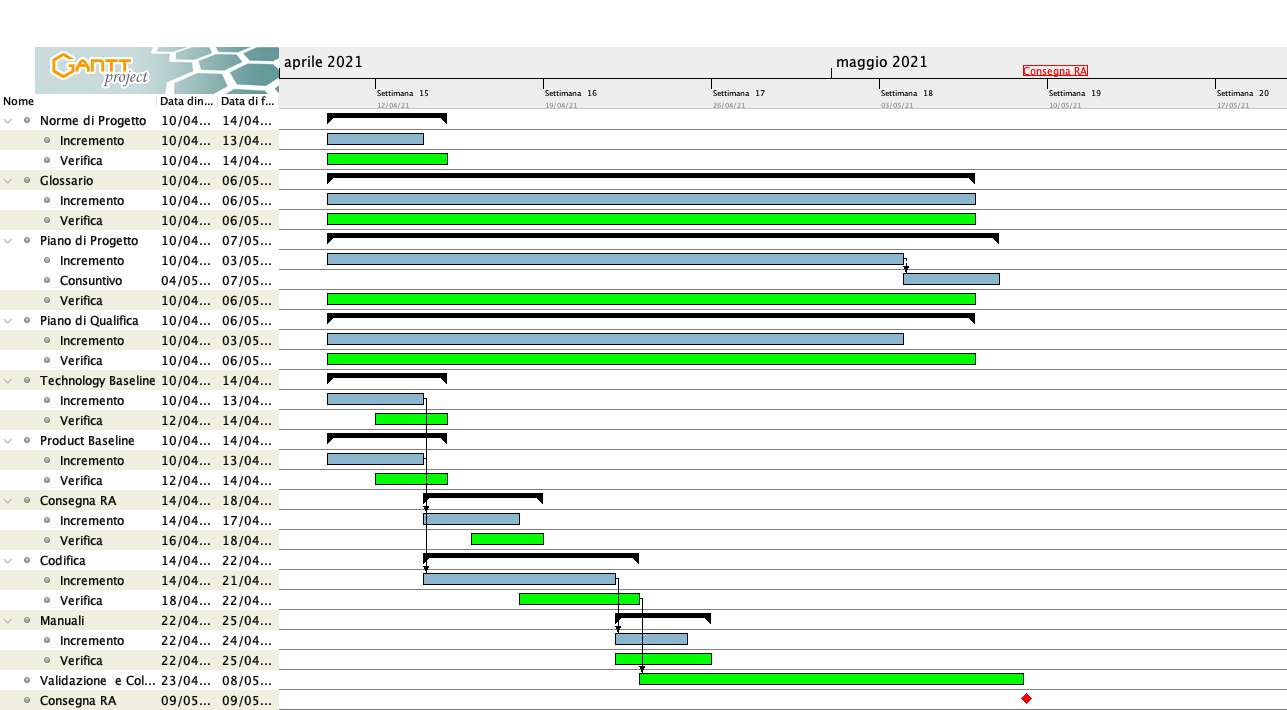
\includegraphics[width=\textwidth]{Immagini/GanttValidazioneECollaudo}
    \caption{Diagramma di Gantt dell'attività di Validazione e Collaudo}
\end{figure}